\chapter{Introduction}
\label{ch:intro}

%Mathematical theorem provers comes equipped with libraries of formalized mathematics. 
A large library of formalized, ready-to-use mathematics has long been the pursuit of mathematicians and computer scientists.  
The influential QED manifesto~\citep{boyer1994qed}, released in 1994, envisioned a library in which all mathematics is formalized and rigorously checked. The QED manifesto believed in one-formalization-fits-all approach to building this library.
Diversity in mathematical formalizations was a big obstacle towards realizing the library described by QED. There was not an agreement even on which foundation to use for formalizing all of mathematics~\cite{qedrealoaded2016}.  Since then, mathematical knowledge management (MKM) has become an active area of research framing a new vision for a large math library. The universal digital math library (UDML), described in~\cite{farmer2004mkm}, is a collection of heterogeneous, intercommunicating systems and building this library is described as a grand challenge facing MKM. 

Despite the many efforts dedicated to building math libraries, a large universal library has not become a reality.\footnote{However, in 2020, the mathlib team is making serious inroads in that direction~\cite{lean2019} .} One reason is that developing and maintaining libraries of mathematics requires a lot of person-power. One would want to believe that this human effort is put into the creative work of formalizing new pieces of knowledge. By examining current libraries of theorem provers, we know this is not always the case. 
Libraries formalizing the algebraic hierarchy have been formalized various times, sometimes even within the same system~\cite{Geuvers2002, Gonthier2009, Spitters2010, coq-contribs-algebra}. 
In every formalization, the library developers had to provide all the definitions of the structures in the hierarchy and related constructions such as homomorphisms. We want to add more automation to the process of building libraries. We identify sources of redundancy that can be eliminated and use the theory of \lstmath{Monoid} as our running example. \lstmath{Monoid} is an algebraic structure, a member of the algebraic hierarchy, that describes algebras with a carrier set and an associative binary operation over that set that has an identity element.
%The libraries for theorem provers contain definitions provided by library developers that . 
%We give examples of redundancies associated with defining the algebraic hierarchy in libraries of formal systems in Chapter~\ref{ch:redundancy}. 
%By investigating the formalization of the algebraic hierarchy in libraries of formal systems, we can see 
%It mainly requires developers to To understand why this redundancy exists, we examine the formalization of \lstmath{Monoid} in algebra textbooks versus in interactive theorem provers. 

\paragraph{Handwritten Boilerplate.}
\lstmath{Monoid} is defined in~\cite{jacobson1985basic} as
\begin{quote}
    A monoid is a triple $(M,p,1)$ in which $M$ is a non-vacuous set, $p$ is an associative binary composition (or product) in $M$, and $1$ is an element of $M$ such that $p(1,a)= a = p(a,1)$ for all $a \in M$ 
\end{quote}
The definition of \lstmath{Monoid} is followed by the definition of its homomorphism as
\begin{quote}
If $M$ and $M^\prime$ are monoids, then a map $\eta$ of $M$ into $M^\prime$ is called a homomorphism if 
\begin{multicols}{3}
    $\eta(ab)=\eta(a)\eta(b)$, \vfill   
    \columnbreak
    $\eta(1) = 1$, \vfill   
    \columnbreak 
    $a,b \in M$  \vfill    
\end{multicols}
\end{quote}
More monoid-related constructions are defined, like submonoid, and quotient monoids. The same constructions are defined for \lstmath{Group} and \lstmath{Ring}. 
%Mathematics presented in textbooks rely on the human understanding to be able to generalize these concepts. For example, \cite{jacobson1985basic} does not provide an explicit definition for group homomorphism, but proceeds to use it. 

Formal systems\footnote{We use the term \emph{formal systems} to refer to all computer systems with logical foundations, be it automatic theorem prover (ATP), interactive theorem prover (ITP), specification system, or others.} present algebraic structures using axiomatic theories. \lstmath{Monoid} and its notion of homomorphism are presented axiomatically in a minimal (imaginary) computer language as follows: \\
\begin{tabular}[t]{p{6.3cm} p{1cm} p{6.3cm}}
\begin{lstlisting}[mathescape, basicstyle=\footnotesize]
theory Monoid { 
  A : type 
  e : A
  op : A $\to$ A $\to$ A
  lunit : {x : A} $\to$ op e x = x 
  runit : {x : A} $\to$ op x e = x 
  assoc : {x y z : A} $\to$ 
      op x (op y z) = op (op x y) z
}
\end{lstlisting}
& &
\begin{lstlisting}[mathescape, basicstyle=\footnotesize]
theory MonoidHom { 
  M1, M2 : Monoid  
  hom : M1.A $\to$ M2.A 
  pres-e : hom (M1.e) = M2.e
  pres-op : (x y : M1.A) $\to$ 
             hom (M1.op x y) = 
             M2.op (hom x) (hom y) }
             
             
             
\end{lstlisting}
\end{tabular}

Let us now define \lstmath{Group} and \lstmath{Group} homomorphism within the same language: \\
\begin{tabular}[t]{p{6.3cm} p{1cm} p{6.3cm}}
\begin{lstlisting}[mathescape, basicstyle=\footnotesize]
theory Group {
  A : type 
  e : A
  op : A $\to$ A $\to$ A
  inv : A $\to$ A
  lunit_e : {x : A} $\to$ op e x = x
  runit_e : {x : A} $\to$ op x e = x
  linverse : {x : A} $\to$ 
          op x (inv x) == e
  rinverse : {x : A} $\to$ 
          op (inv x) x == e
  assoc : {x y z : A} $\to$ 
          op x (op y z) = op (op x y) z }
\end{lstlisting}
& &
\begin{lstlisting}[mathescape, basicstyle=\footnotesize]
theory GroupHom { 
  G1, G2 : Group 
  hom : G1.A $\to$ G2.A
  pres-e : hom (G1.e) = G2.e
  pres-op : (x y : G1.A) $\to$ 
            hom (G1.op x y) = 
            G2.op (hom x) (hom y)
  pres-inv : (x : G1.A) $\to$ 
            hom (G1.inv x) = 
            G2.inv (hom x)  }
\end{lstlisting}
\end{tabular}

Notice how the two definitions of homomorphisms are similar and depend uniformly on the details of the theory. This observation is not specific to \lstmath{Monoid} and \lstmath{Group}. Generally, the homomorphism of a theory \lstmath{X} is a mapping between two instances (algebras) of \lstmath{X} and has $3$ components: 1) the two instances of the theory, 2) the function \lstmath{hom} that maps the carriers of the $2$ instances, and 3) a preservation axiom \lstmath{pres-op} for each operation symbol \lstmath{op}. The preservation axioms follow the pattern
\begin{lstlisting}[mathescape]
{x$_1$ .. x$_n$ $\in$ A$_1$} $\to$ hom (op$_1$ x$_1$ .. x$_n$) = op$_2$ (hom x$_1$) .. (hom x$_n$)
\end{lstlisting}
where \lstmath{A$_1$} is the carrier of the first instance and the domain of the \lstmath{hom} function. \lstmath{op$_1$} and \lstmath{op$_2$} are the instances of the function symbol \lstmath{op} residing in the first and the second instances, respectively. 

This definition of homomorphism is given to us by universal algebra~\cite{whitehead1898treatise}, which studies commonalities between algebraic structures and define their related constructions.
%\lstmath{Monoid} and \lstmath{Group} are two of many algebraic structures used in abstract algebra. The commonalities between these structures is the subject of study of universal algebra, 
It defines an algebra as~\cite{mckenzie1987algebras}\footnote{An axiomatic theory that describes an algebra will also have a field in the ordered pair for the axioms describing its properties.}: 
\begin{quote}
    An algebra is an ordered pair $\langle A, F \rangle$ such that $A$ is a nonempty set and $F = \langle F_i : i \in I \rangle$ where $F_i$ is a finitary operation on $A$ for each $i \in I$. $A$ is called the universe of $\langle A, F \rangle$, $F_i$ is referred to as a fundamental or basic operation of $\langle A, F \rangle$ for each $i \in I$, and $I$ is called the index set of the set of operation symbols for $\langle A, F \rangle$. 
\end{quote}
%\ednote{look for a text book that explicitly state axioms. The properties of the function symbols, which are mentioned in mathematics textbooks but not always stated, are stated as axioms in formal systems, and so we defined an algebraic theory to be a type ($\langle A, F \rangle$,$E$), where $E$ is the set of axioms.}
%\todo{check the sanella software specification book for this definition. }
Libraries formalizing the algebraic hierarchy would contain axiomatic theories describing algebras and their related constructions, like homomorphism, subalgebra, quotient algebra, term language, etc. 
For every one of those constructions, universal algebra provides a uniform definition in terms of the components of the theory. 
It gives us the meta theory and the abstractions that enables us to instantiate those definitions for every theory. This suggests that we can have a program generate those constructions from the individual theories, instead of having library developers provide them manually. As there are many algebraic structures in mathematics and computer science and many constructions for each of them, this automation can save significant human effort. In this work, we provide a framework for generating these constructions. 
%There are many algebraic structures and many constructions related to each of them. Their definitions are part of libraries of algebra in formal systems. Universal algebra provides a strong meta-theory for abstracting over the details of those structures and their related constructions. In this work, we want to use those abstractions to define algorithms that given a theory would compute the constructions. 

\paragraph{Variabilities in Theory Presentations.}
Universal algebra gives us the right abstractions to implement the generation framework, but we need to start with a choice of a theory presentation from which the constructions will be computed. We have shown the definition of \lstmath{Monoid} in an imaginary language. But formal systems have different ways to define \lstmath{Monoid}. 
In Figure~\ref{fig:mon-diff-lang}, we show the definitions of \lstmath{Monoid} in $5$ different language. 
\begin{figure}
    \footnotesize
\begin{tabular}{p{6.3cm} p{7cm}}
\underline{Haskell}
\begin{minted}[mathescape]{haskell}
class Semigroup a => 
      Monoid a 
 where 
  mempty :: a 
  mappend :: a -> a -> a 
  mappend = (<>) 
  mconcat :: [a] -> a 
  mconcat = 
   foldr mappend mempty 
\end{minted} 
\underline{Lean}
\begin{leancode}
class monoid (M : Type u)
 extends semigroup M, 
         has_one M :=
  (one_mul : ~$\forall$~ a : M, 
           1 * a = a) 
  (mul_one : ~$\forall$~ a : M, 
           a * 1 = a)   
\end{leancode} 
% [mathescape=true, escape_inside=~~]
\underline{Coq}
\begin{minted}[mathescape=true, escapeinside=~~]{coq}
class Monoid {A : type}
 (dot : A ~$\to$~ A ~$\to$~ A)
 (one : A) : Prop := {
  dot_assoc : 
   forall x y z : A, 
   (dot x (dot y z)) = 
   dot (dot x y) z
  unit_left : forall x, 
   dot one x = x 
  unit_right : forall x, 
   dot x one = x              
}
~$\text{\textit{Alternative Definition:}}$~
Record monoid := {
 dom : Type; 
 op : dom -> dom -> dom 
  where "x * y" := op x y; 
 id : dom where "1" := id; 
 assoc : forall x y z, 
  x * (y * z) = (x * y) * z; 
 left_neutral : forall x,   
  1 * x = x; 
 right_neutal : forall x,
  x * 1 = x; 
}
\end{minted} 
&
\underline{Agda}
\begin{agdacode}
record Monoid c ~$\ell$~ : 
   Set (suc (c ~$\sqcup$~ ~$\ell$~)) where 
 infixl 7 _~$\bullet$~_
 infix 4 _~$\approx$~_
 field 
  Carrier : Set c 
  _~$\approx$~_ : Rel Carrier ~$\ell$~ 
  _~$\bullet$~_ : Op~$_2$~ Carrier 
  isMonoid : IsMonoid _~$\approx$~_ _~$\bullet$~_ ~$\varepsilon$~ 
  
record IsMonid (~$\bullet$~ : Op~$_2$~) (~$\varepsilon$~ : A) 
 : Set (a ~$\sqcup$~ ~$\ell$~) where 
  field 
   isSemiring : IsSemiring ~$\bullet$~ 
   identity : Identity ~$\varepsilon$~ 
       
   open IsSemigroup isSemigroup public 
   
   identity~$^l$~ : LeftIdentity ~$\varepsilon$~ ~$\bullet$~ 
   identity~$^l$~ = proj~$_1$~ identity 
   identity~$^r$~ : Rightdentity ~$\varepsilon$~ ~$\bullet$~ 
   identity~$^r$~ = proj~$_2$~ identity        
\end{agdacode}       
\underline{MMT}
\begin{minted}[mathescape=true, escapeinside=~~]{mmt} 
theory Semigroup : ?NatDed = 
 u : sort 
 comp : tm u ~$\to$~ tm u ~$\to$~ tm u 
  # 1 * 2 prec 40
 assoc : ~$\vdash$~ ~$\forall$~ [x, y, z]
  (x * y) * z = x * (y * z)    
 assocLeftToRight : 
  {x,y,z} ~$\vdash$~ (x * y) * z 
          = x * (y * z) 
  = [x,y,z] 
   allE (allE (allE assoc x) y) z
 assocRightToLeft : 
  {x,y,z} ~$\vdash$~  x * (y * z) 
           = (x * y) * z 
  = [x,y,z] sym assocLR 
theory Monoid : ?NatDed 
 includes ?Semigroup 
 unit : tm u # e 
 unit_axiom : ~$\vdash$~ ~$\forall$~ [x] = x * e = x       
\end{minted}      
\end{tabular}  

    \caption{Representation of \lstinline|Monoid| theory in different languages.}
    \label{fig:mon-diff-lang}
\end{figure}
The $5$ definitions refer to the same mathematical concept, but they look very different. 
Each one has all the components needed to describe a \verb|Monoid|. Yet, they also reflect the design decisions taken by the library developers. 
For example, the Haskell and MMT definitions exposes the fact that \monoid in these libraries is defined as an extension of \semigroup. This forces users of the definition to deal with \semigroup theory even if their formalization does not need to. 
%the theory \monoid is defined as an extension of \semigroup. Despite this being useful, there is no reason why a developer might not want to add a theory \unital (a non-associative \monoid), to the hierarchy. Exposing this hierarchy to the user makes their code vulnerable in case the hierarchy changes. This problem occurred when Haskell changed the hierarchy of type classes when \lstmath{Applicative} became a superclass for \lstmath{Monad} ~\cite{wiki:haskell_hierarch}. The work in \cite{cohen2020hierarchy} discusses this problem. 
The two Coq definitions takes two extreme views to the bundling problem~\cite{lean2019,alhassy2019,spitters2011type} by either having the carrier and all the function symbols as arguments (the first definition) or having all elements of the theory as declarations of a record type (the second definition). 
The formalization of the Algebraic hierarchy in the Agda standard library is based on setoids (sets equipped with an equivalence relation). Therefore, we find an extra field of the definition of \monoid corresponding to the equivalence relation $\_\approx\_$. 

Having design decisions embedded into the library definitions is a big usability problem. Users won't be able to use them in their projects unless they employ the same decisions. Otherwise, they are forced to redefine them. That leads to many libraries formalizing the same knowledge, even in the same language. Coq has at least $4$ different algebra libraries~\cite{Gonthier2009,Geuvers2002,Spitters2010,coq-contribs-algebra}. In~\cite{Gonthier2009}, the authors acknowledge this situation saying:  
\begin{quote}
    ``In spite of this body of prior work, however, we have found it
    difficult to make practical use of the algebraic hierarchy in our project to
    formalize the Feit-Thompson Theorem in the Coq system."
\end{quote}

We seek to use a generative approach to building libraries that would compute derivable information from a theory presentation. We want to abstract over design decisions, so our generated definitions become accessible to more platforms and user projects.  
%We want to abstract over design decisionsIn this work, we This kind of redundancy is addressed in this thesis using generative programming. We define an abstraction over design decisions, from which different constructions defined by universal algebra can be automatically generated. By minimizing the design decisions that are embedded into the definition we aim to reduce redundancy and increase usability. 



\begin{comment}
\begin{itemize}
\item[Q3] What tools are needed to generate this information?  
\end{itemize}
We need a language to capture the abstractions of universal algebra, and meta programming capabilities to enable manipulating them to automatically generate new ones. 

When choosing the language, we don't want to be burdened with system-specifc details. We want to be as system independent as possible, as our ideas should apply to all systems that are able to represent first order theories. We see in Figure XX that normal practice of theory definition in many systems have design decisions embedded in the definition of the theory. We choose Tog~\cite{tog}, a minimal dependently types system to implement our ideas. We introduce it in Chapter~\ref{ch:tog}.  
\end{comment}

\section{Research Problem}
\label{sec:questions}
%Our work contributes to the efforts of building large library of mathematics. We want to reduce the human effort needed to build such libraries by employing generative programming. 

%\begin{itemize}
%\item[O1:] Some constructions related to algebra can be automatically generated by manipulating theory presentations describing the algebras on the bases of universal algebra definitions. 
%\item[O2:] 
%\end{itemize}

We want to enhance the process of library development. Instead of having library developers provide every piece of detail in the library, we want to employ a generative approach to the development. The library developers would be providing expressions describing the definitions to be included. 
Our generator would produce those definitions. 

We believe a generative approach is possible because definitions within a library are written in formal languages which provide uniform syntax for expressing information and universal algebra provides the definitions of many constructions in terms of the components of the algebraic structure. 

 A generative approach would have the following benefits: 
\begin{itemize}
    \item Reduce the human effort put into producing standard knowledge by internalizing this knowledge in the generator.
    \item Enhance the library maintainability. Library developers write generative algorithms to create and manipulate definitions. Changing design decisions leads to changes in the generative algorithm. 
    \item Increase the usability of library definitions by reducing the amount of design decisions embedded into them. 
\end{itemize}  

%The problem we are solving is that libraries of algebra have handwritten boilerplate provided by the library developers. Providing these definitions increases the human effort needed to build the library. On the other hand, we know that the right abstractions needed to generate those definitions have been well studied in universal algebra. This suggests that we can have algorithms that manipulate definitions of structures to produce definitions of their related constructions. 

%We have highlighted two sources of 

%By investigating definitions in algebra libraries, we find that there are two sources of redundancies We define two sources of redundancy in algebra libraries 
%\begin{itemize}
%    \item Handwritten library definitions that can be automatically generated by manipulating the definitions of the algebraic structures. 
%    \item Variabilities in theory presentations across the different formal systems due to the different design decisions they employ. 
%\end{itemize}


%This human work can be saved if universal algebra can be used to \emph{generate} some definitions. Many problems face this generative approach, some are 1) having design decisions baked into library definitions makes universal algebra abstractions not directly applicable, 2) Manipulating definitions require going to the meta-level using either strong reflection mechanisms or meta programs in the host language 

%We suggest a generative approach in which a developer can \emph{describe} the information they need in the library and the design decisions they are employing, then library definitions get generated based on this description. This way we provide a domain specific langage (DSL) for theory development\ednote{introduce theory development}. 
%\ednote{talk more about DSLs and why they are used}. 
%It would lift the burden of having to define utilities that are needed to perform the task in hand, but are standard information to the point that writing them is boring and distracting from the original task. 
%The DSL approach is useful in various ways. First, providing well-studied combinators to build algebraic theories can elevate their structure and connect them the right way, as we discuss in chapter~\cite{ch:library}. Also, library developers can use this DSL to generate parts of their library. Last, users of formal systems can use this DSL to automatically create utilities they need to get the systematic stuff done and focus on the novelty of their task. 

We are inspired by the \emph{deriving} mechanism in Haskell. When defining a new datatype, a Haskell user can ask for some utilities to be readily available for them to use on that type. The Haskell compiler would then generate these functions for the user. Some of these are basic, like equality and printer, but the community has gone as far as giving users the chance to define their own templates for deriving instances, knows as the \emph{deriving-via} technique~\cite{loeh2018derivingVia}. A pretty impressive example of deriving information is shown in Figure~\ref{fig:deriving-via-example}. 
Also, the Lens library~\cite{lensesLib} in Haskell, uses Template Haskell~\cite{sheard2002TH} for the same purpose. 
\begin{figure}
    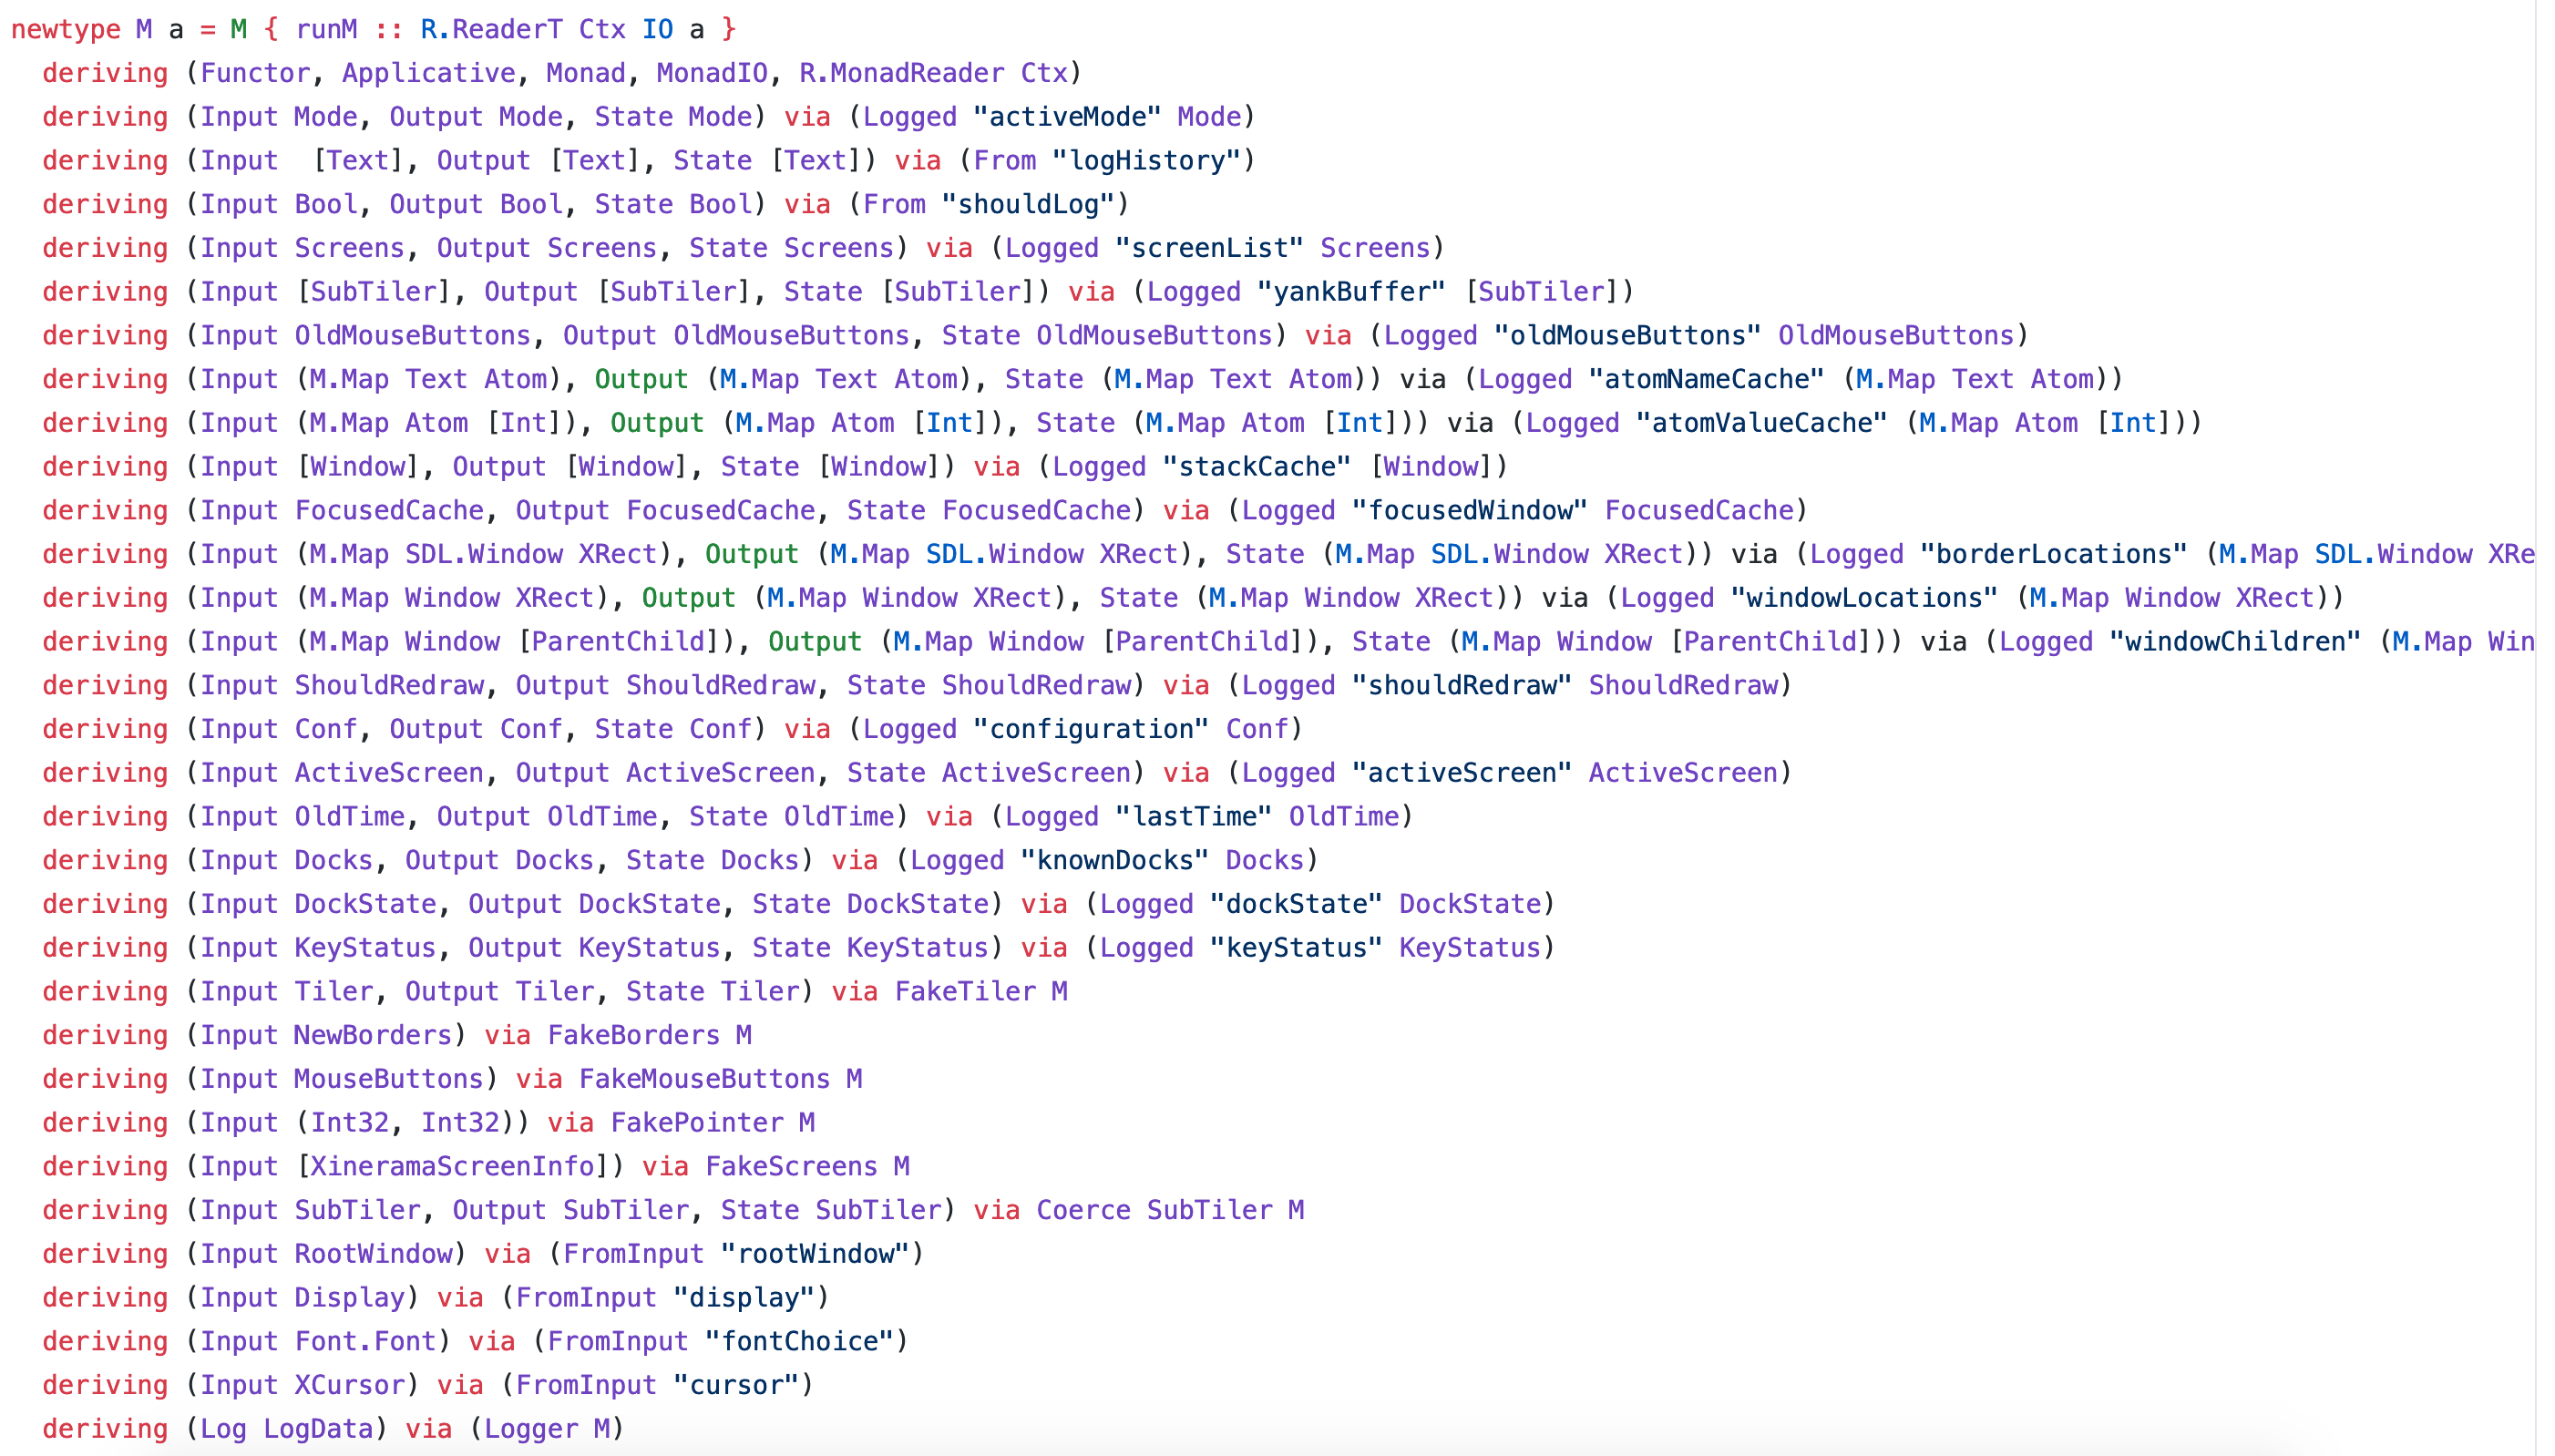
\includegraphics[scale=0.5,width=\linewidth]{figures/deriving-via-example.png}
    \caption{Example of deriving information in Haskell. \\ source: \href{https://github.com/jhgarner/Xest-Window-Manager/blob/3741b35a69eb2cf8cd7320e186fd40134d1c1a56/src/Base/DoAll.hs}{Xest Window Manager Project} on github.}
    \label{fig:deriving-via-example}
\end{figure}

%The definitions we use in our development are based on universal algebra abstractions. Universal algebra abstracts over algebraic structures and their related constructions and provides the meta theory that explains how the generation algorithms should work. A theory presentation in universal algebra has three components \verb|(S,F,E)|; a sort \verb|S|, a list of function symbols along with their types \verb|F|, and a list of axioms (equations) that describe properties of the function symbols \verb|E|. If we can abstract over the details of theory presentations to extract this information, we are able to generate the constructions defined by universal algebra, like morphisms, product algebras, term languages, and others. 

In this work, we address the following research questions
\begin{enumerate}
    \item[RQ1] Can the uniformity provided by universal algebra be captured by a meta program that generates parts of an algebra library? 
    \item[RQ2] What are the preconditions for generating this new information? 
%    \item[RQ3] Which information need to be provided by the developer and which ones can be generated?     
    \item[RQ3] What design decisions can be abstracted away and which can be reintroduced after the generation of new constructs?
    \item[RQ4] How would this affect the activity of library building?
    \item[RQ5] Can these generative algorithms be extended beyond the structure captured by universal algebra? 
\end{enumerate}

\section{Contributions}
These are the principle contributions of the thesis: 
\begin{itemize}
    \item Highlight the redundancy in libraries formalizing the algebraic hierarchy (in Chapter~\ref{ch:redundancy}). 
    \item Build a library of over $200$ theories describing the algebraic hierarchy, implemented using the combinators in~\cite{carette2018building} (Chapter~\ref{ch:library}). 
    \item Compile a list of structures that can be generated from theory presentations (Section~\ref{sec:toBeGenerated}). 
    \item Generate some of these constructions in Tog, a small implementation of a dependently typed language, in the style of Agda, Coq and Lean (Chapter~\ref{ch:generation}). 
    \item Export this implementation to Agda, (Chapter~\ref{ch:export}). 
\end{itemize}  

\section{Broader Context}
\label{sec:broader_context}
%Our aim to support building large libraries contributes to 
%work fits in the effort of building a
The Tetrapod project~\cite{carette2020bigMath} envisions a software system in which $5$ aspects of doing mathematics are integrated. These $5$ aspects are organization, inference, computation, narration, and concretization. The system will have a tetrapodal structure with knowledge organization in the center and each of the $4$ modes making one of the legs of the tetrapod, as shown in Figure~\ref{fig:tetrapod}. 
\begin{figure}[h]
\centering{
\begin{tikzpicture}[scale=\myscale]
  \node (center) at (0,.15) {Organization};
  \node (left) at (.2,-.3) {Computation};
  \node (right) at (.4,0) {Inference};
  \node (back) at (-.5,0) {Narration};
  \node (up) at (0,.5) {Concretization};

  \draw[very thick] (center) -- (left);
  \draw[very thick] (center) -- (right);
  \draw[very thick] (center) -- (back);
  \draw[very thick] (center) -- (up);
  \draw[dotted] (left) -- (right) -- (back) -- (left);
  \draw[dotted] (up) -- (left);
  \draw[dotted] (up) -- (right);
  \draw[dotted] (up) -- (back);
\end{tikzpicture}}
\caption{The tetrapodal structure of a mathematical software system that supports the five aspects of doing mathematics. }
\label{fig:tetrapod}
\end{figure}

The organization aspect is reflected in the efforts of building libraries of mathematics. The Tetrapod project supports building a large library of mathematical knowledge organized as theory graph of biform theories~\cite{biformCICM2018}. The theory graph structure connects theories by describing how the symbols of a source theory can be interpreted in the target one. In a graph, one can express facts like `a group is a monoid` and that `monoid and additive monoid are isomorphic`. We explain theories, morphisms and graphs in more details in Chapter~\ref{ch:background}. 
Ideally, we want the nodes of the theory graph to be biform theories~\cite{biformCICM2018} which connect axiomatic theories  (used by theorem provers) and algorithmic theories (used by computer algebra systems) using meaning formulas. This way communication between reasoning and computation systems becomes possible. Communication can take the form of reasoning about algorithmic theories or using results of computer algebra systems in theorem provers.

This work contributes to the Tetrapod project by investigating how a generative approach can contribute to building the library at the center of the tetrapod. We focus on building the algebraic hierarchy and the constructions related to the theories in it, mainly as described by universal algebra. The library we build has a theory graph structure, but the nodes are axiomatic, rather than biform, theories. 
%The theories we consider here are axiomatic theroies. that automatically generates a theory graph from theory expressions described in~\cite{carette2018building}. The nodes of this graph are axiomatic theories. We then work on the nodes of the graph to extract information from them. Finally, we make this information available in a agda. 
%There are different ways of organizing knowledge within a formal system. Our work contributes to building a large math library organized as a theory graph in the heart of a tetrapodal structure. Theory graphs, explained in details in Section~\ref{sec:background:theorygraph}, capture the structure of mathematical knowledge by enabling the description of relationships between the different pieces using morphisms. Using them, we can express facts like `a group is a monoid` and that `monoid and additive monoid are isomorphic`. 

%The nodes of a theory graph can be any kind of theories. Ideally, they would be biform theories~, as they connect axiomatic theories

%Morphisms are meaning preservation maps. The simplest form of a morphism is inclusion. Morphisms are used to transfer results from one theory to another. So, a morphism between \lstmath{Monoid} and \lstmath{AdditiveMonoid} that describes they are isomorphic, allows us to transfer results between them. 

%In, the authors argue that modern mathematics is organized as a tetrapod with knowledge organization being at its center. We are working towards a library organized as a theory graph of biform theories that serves as this center. Different aspects of the tetrapod will be consumers and producers of knowledge in this library. This implies that the size of this library would be huge, and that using generative approach to support its building would be a great asset. 

%We support the building of this library by providing combinators to define the library theories and algorithms to compute related constructions

\section{Publications}
This thesis lead to the following publications: 
\begin{itemize}
    \item \cite{biformCICM2018} 
        \begin{itemize}
        \item[] Contributed to writing the project description of biform theories, mainly the motivation. The project description appeared in the proceedings of CICM 2018. 
        \end{itemize}
    \item \cite{carette2018building} 
    \begin{itemize} 
    \item[] Contibuted to an extended paper discussing the MathScheme combinators that were initially published in~\cite{CaretteOConnorTPC}. The extended paper has been submitted to the \textit{Journal of Automated Reasoning}. I contributed to surveying related work and framing the novelty of the work with respect to this related work, developing the type systems for the combinators, and implementing them as discussed here in Section~\ref{sec:lib_implementation}. I used this implementation to build a revised version of the MathScheme library. 
    %The development of the initial version of the library was part of the experiments~\cite{mathscheme2011experiments} that lead to the development of the combinators. To rebuild the library, we put some effort towards redefining the definitions that went wrong in the experiments. I also took part in developing the type systems for the combinators. 
%Surveying theory expressions in different formal systems to frame the novelty of the paper. 
%Taking part in developing the type system for the combinators 
%Providing the first arrow-based implementation of the paper, as we discuss in Section~\ref{sec:lib_implementation}. 
%Using the combinators to build a library of over $200$ theories. Although the library definitions pre-existed, many of them were not correct because they were based on theories. Shifting the implementation to arrows mandated figuring out the right arrows to build the theories, which was never done before this work.
   \end{itemize}
    \item ~\cite{cicm2019diagrams} 
    \begin{itemize}
    \item[] Used the diagram infrastructure developed in MMT~\cite{rabe2013scalable} and described in the paper to implement the MathScheme combinators described in~\cite{carette2018building}. Since the combinators compute a theory and some arrows, we considered treating their inputs and outputs as diagrams.
This was an earlier attempt to implement the combinators and also the first time diagrams combinators in MMT were tested.  There were promising results, but they did not scale up since --- at that time --- there were problems with how MMT supports the diagram combinators. 
    \end{itemize}        
    \item \cite{cicm2019docotral} 
    \begin{itemize}
    \item[] Extended abstract submitted to the Doctoral Program at CICM 2019. The abstract was presented in the conference, but not refereed. 
    \end{itemize}
    \item \cite{leverageCICM2020} 
    \begin{itemize}
    \item[]  Presented redundancy in existing libraries and highlighted some of the problems we tackle in this thesis. Some of the main results of this thesis are published in the paper. I collected the examples of redundancy, and implemented and tested the framework.
    \end{itemize} 
    \item \cite{bercic2020space} (preprint)
    \begin{itemize}
    \item[] Contributed to surveying and categorizing how different mathematics software organize knowledge. Knowledge organization is one of $5$ categories of mathematics software the paper surveys. The other $4$ are inference, computation, concretization, and narration. 
%    The paper introduces a tetrapodal  organization of knowledge is in the cent paper discusses software used by producers and consumers of mathematical knowledge. 
    \end{itemize}        
\end{itemize}

\section{Outline}
We start by introducing some background knowledge in Chapter~\ref{ch:background}. 
We introduce universal algebra and the constructions of interest to this work in Chapter~\ref{ch:ualgebra}. 
We give in Chapter~\ref{ch:redundancy} examples of how some of these constructions are currently presented in libraries of formal systems, highlighting the redundancies that can be avoided.
We present Tog, the language and type checker that we use to develop our framework in Chapter~\ref{ch:tog}. 
In Chapter~\ref{ch:design}, we introduce the methodology we use to enhance the library development process. 
We discuss how we extend Tog to support combinators for building the algebraic hierarchy in Chapter~\ref{ch:library}. 
In Chapter~\ref{ch:generation}, we discuss our generative framework that computes the constructions related to a specific theory.  
The theories and the generated constructions are exported to Agda. We discuss the exporter in Chapter~\ref{ch:export}. 
We present related work in Chapter~\ref{ch:relatedwork}. Conclusions and future work are discussed in Chapter~\ref{ch:conclusion}. 
\ednote{always check that this description of chapters still hold} 
